\documentclass[a4paper, 12pt]{scrartcl}

\usepackage[utf8]{inputenc}
%\usepackage[ngerman]{babel}
\usepackage[T1]{fontenc}
\usepackage{amsmath}
\usepackage{braket}
\usepackage{amssymb}
\usepackage{graphicx}
\usepackage{wrapfig}
\usepackage{hyperref}


\author{Sebastian Steinhäuser}

\begin{document}

\begin{center}
\Large{\textbf{Spezialisierungsbericht}}
\\
\vspace{1cm}
\Huge{\textbf{Computersimulation aktiver Random-Walks auf perkolierendem Cluster}}
\\
\vspace{1cm}
\Large{Sebastian Steinhäuser}

\includegraphics[width=0.75\textwidth]{DLR.jpg}
\end{center}
\begin{center}
Betreut durch Thomas Voigtmann und Julian Reichert
\end{center}
\newpage
\tableofcontents
\newpage
\section{Perkolation}
\subsection{Was ist Perkolation?}
In diesem Bericht geht es um Perkolation und vor allem um den Random-Walk (mathematisches Modell für eine Bewegung, bei der die einzelnen Schritte zufällig erfolgen) auf einem perkolierenden Cluster in einem Quadratgitter in zwei Raumdimensionen. In diesem Fall gibt es zwei geläufige Perkolationsmodelle, Knotenperkolation (engl. 'site-percolation') und Kantenperkolation (engl. 'bond-percolation'), hier wird immer über Knotenperkolation gesprochen. In folgender Abbildung wird der Unterschied zwischen Knoten- und Kantenperkolation bildlich dargestellt \footnote{https://de.wikipedia.org/wiki/Perkolationstheorie, 21.10.2019}.
\begin{figure}[h!]
\centering
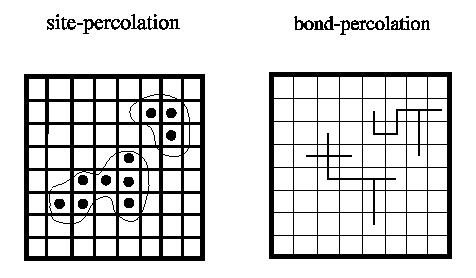
\includegraphics[scale=0.6]{Percolation1.jpg}
\caption{Knoten- und Kantenperkolation}
\end{figure}
\vspace{0,5cm}
\\
Das Quadratgitter wird zufällig mit einer Wahrscheinlichkeit $1-p$ geblockt. Es ist Konvention, die Wahrscheinlichkeit, dass ein Platz frei ist, mit $p$ zu bezeichnen, diese Konvention möchte ich hier erhalten. Geblockte Plätze können nicht besetzt werden. Man kann sich geblockte Plätze wie Wände eines Labyrinths vorstellen, durch die der Random-Walker später nicht hindurch kommt.  
\\
Nun definiert man einen Cluster als eine Gruppe benachbarter Quadrate die begehbar sind, also nicht geblockt. Man nennt einen Cluster perkolierend, wenn sich der Cluster von einer Kante zur gegenüberliegenden Kante erstreckt, so dass zum Beispiel Wasser durch das Gitter fließen könnte, ähnlich wie es durch eine Kaffeemaschiene (engl. 'percolator') perkoliert/sickert. Vereinfacht gesagt kann ein Random-Walker auf dem perkolierenden Cluster sich unendlich ausbreiten und ist nicht 'eingesperrt'. Man kann sich nun leicht Vorstellen, dass wenn kaum Felder geblockt sind (also $p$ nahe $1$) sich auf dem (unendlich großen) Quadratgitter stets ein perkolierender Cluster finden lässt und wenn kaum Felder begehbar sind (also $p$ nahe $0$) sich nie ein perkolierender Cluster finden lässt. Es gibt dazwischen eine sogenannten kritischen Wert $p=p_c \approx 0.5928$ \footnote{D. Stauffer, Perkolationstheorie (Taylor \& Francis, London, 1994)} bis zu welchem das unendliche Quadratgitter perkoliert, auch Perkolationsschwelle oder englisch percolation-threshold genannt.
\noindent Historisch geht die Perkolationstheorie (engl. 'percolation theory') auf Paul Flory und Walter H. Stockmayer zurück, die sie während des Zweiten Weltkriegs entwickelten, um Polymerisationsprozesse zu beschreiben. Der Polymerisationsprozess kommt durch das Aneinanderreihen von Molekülen zustande, die dadurch Makromoleküle bilden. Der Verbund solcher Makromoleküle führt zu einem Netzwerk von Verbindungen, die sich durch das ganze System ziehen können.\footnote[1]{Zitiert aus: https://de.wikipedia.org/wiki/Perkolationstheorie, 21.10.2019}
\\
\noindent Üblicherweise wird der Beginn der Perkolationstheorie mit einer Publikation von Broadbent  und Hammersley aus dem Jahre 1957 in Verbindung gebracht, in welcher der Name eingeführt wurde, und in welcher sie mit den oben erläuterten geometrischen und wahrscheinlichkeitstheoretischen Konzepten mathematischer behandelt wurde. Hammersley erwähnt in seiner persönlichen Geschichte der Perkolation in 'Percolation Structures and Processes', dass die (damals) neuen Computer, die für die Wissenschaftler dieser Zeit zugänglich wurden, einer der Gründe für die Entwicklung der Perkolationstheorie waren: Hier handelte es sich um Probleme, bei denen die Computer nützlich werden konnten.\footnote[2]{Zitiert aus: D. Stauffer, Perkolationstheorie}

\subsection{Perkolation auf dem Computer}
Es ist selbstverständlich nicht möglich ein unendlich großes Quadratgitter mit zufällig geblockten und freien Gitterplätzen auf dem Computer zu erzeugen, daher wird hier stets ein endliches Quadratgitter(auf dem Computer in Form einer Matrix/Array gespeichert) und mit periodischen Randbedingungen ausgestattet. Um perkolierende Cluster dieser zufällig erzeugten Matrix zu finden nutzt man den sogenannten Hoshen-Kopelmann-Algorithmus.\footnote[3]{https://www.ocf.berkeley.edu/~fricke/projects/hoshenkopelman/hoshenkopelman.html, 21.10.2019}
Dieser Algorithmus lässt sich am besten an einem Beipiel erklären. Im nachfolgenden Bild sind freie Felder grau und geblockte Felder weiß, graue Felder die an einer Kante verbunden sind (wo der Random-Walker also von einem Feld ins andere kann) werden mit dem selben Label versehen.
\begin{figure}[h!]
\centering
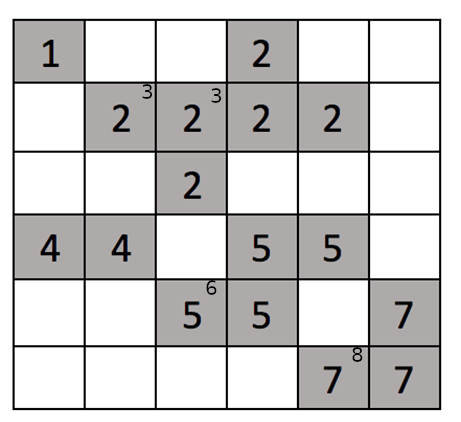
\includegraphics[scale=0.5]{H-K_algorithm.png}
\caption{Veranschaulichung des Hoshen-Kopelmann-Algorithmus}
\end{figure}

\newpage
\subsubsection{Implementierung des Hoshen-Kopelmann-Algorithmus}
Die Idee, wie man dieses anschauliche Nummerieren auf den Computer überträgt ist es, die Matrix von (zum Beispiel) oben links beginnend abzugehen. Stößt man auf ein begehbares Feld (also einen Eintrag $1$ in der Matrix) vergleicht man mit dem Label über und links von diesem Feld, haben beide das selbe Label, so wird dieses auch in das Feld, welches aktuell bearbeitet wird, eingetragen; haben die beiden Felder ein unterschiedliches Label, so merkt man sich in einer Liste, dass diese beiden Label jetzt verbunden sind durch das aktuell zu bearbeitende Feld und später zusammengefügt werden müssen. Sind die Felder oben und links von dem zu bearbeitenden Feld geblockt, so labelt man das Feld mit dem nächst größeren noch nicht benutzten Label. Ist man in diesem Verfahren durch die Matrix durch, so fügt man die verlinkten Labels zusammen; es gilt als Konvention das kleinst mögliche Label zu verwenden. Zum Beispiel verlinkt das vierte Feld der zweiten Reihe in obiger Abbildung 2 die Labels 2 und 3 oder das vierte Feld der fünften Reihe die Labels 5 und 6.
\noindent In python ist dieser Algorithmus für das Labeling (welcher auch in der Bildverarbeitung genutzt wird) bereits in der $scipy.ndimage$ Bibliothek als $measurements$ vorhanden. Nachfolgende Grafik zeigt einen Pseudocode\footnote[3]{https://www.ocf.berkeley.edu/~fricke/projects/hoshenkopelman/hoshenkopelman.html} des Hoshen-Kopelmann-Algorithmus, man kann schön die Unterteilung in scannen des Clusters, verlinken von Labeln (union) und finden der Equivalenzklasse (des Labels) (find) sehen.\newpage

\begin{figure}
	\centering
	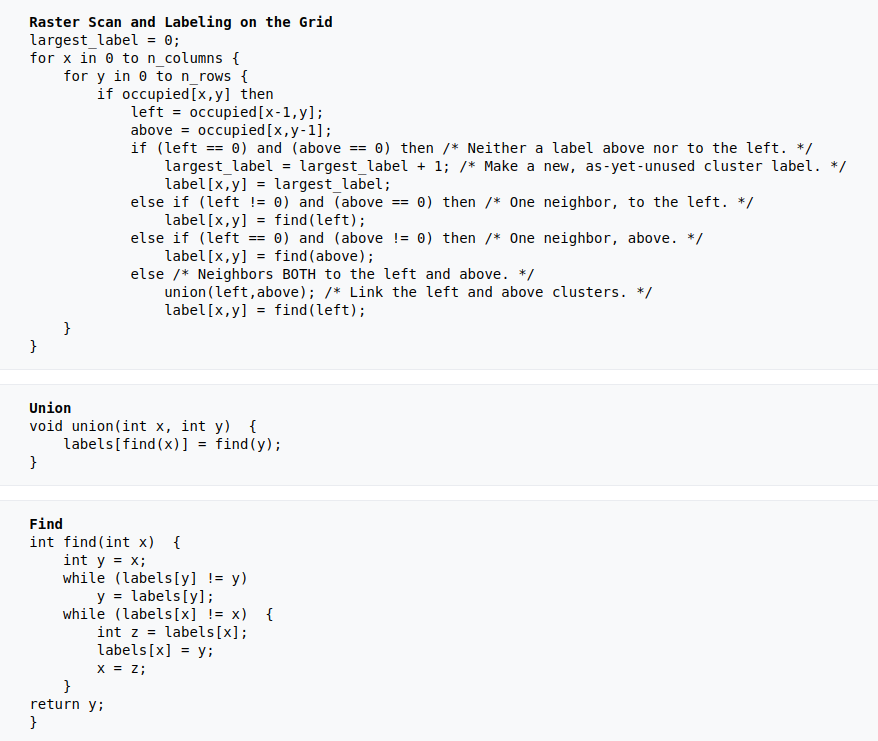
\includegraphics[scale=0.7]{HSK_pseudocode.png}
	\caption{Pseudocode des Hoshen-Kopelmann-Algorithmus}
\end{figure}

\
\subsubsection{Finden von gerichtet perkolierender Clustern}Geht ein Cluster von einem Rand zum gegenüberliegenden Rand, also tritt an diesen beiden Kanten das selbe Label auf so perkoliert dieser Cluster in der endlichen Matrix. Durch die periodischen Randbedingungen muss das Label am gegenüberliegenden Rand in der gleichen 'Höhe' auftreten. Es wird also einfach der linke Rand der Matrix abgegangen und das jeweilige Label mit dem Label an dem rechten Rand verglichen. Analog verfährt man mit dem oberen Rand. Diese Möglichkeit der Perkolation ist durch die periodischen Randbedingungen allerdings nicht die einzige, wie das nächste Unterunterkapitel zeigt.

\subsubsection{Diagonal perkolierende Cluster}
\begin{figure}[h!]
	\centering
	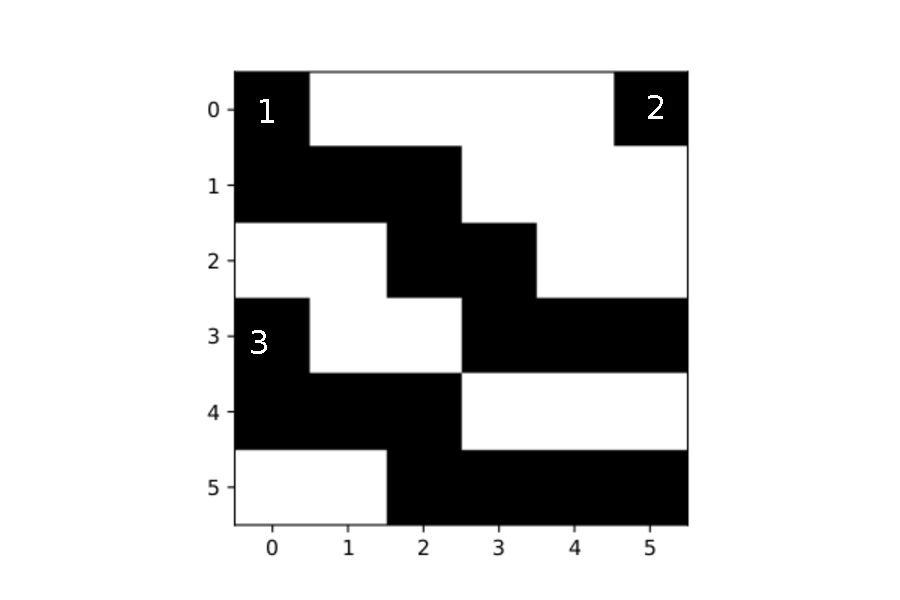
\includegraphics[scale=0.6]{diagonalperc1.pdf}
	\caption{Beispiel eines diagonal perkolierenden Clusters}
\end{figure}
\vspace{0,5cm}
\noindent Neben den in §1.2.2 beschriebenen gerichtet perkolierenden Clustern existieren noch Custer die diagonal über die periodischen Randbedingungen perkolieren. Ein Beispiel ist in Abbildung 4 zu sehen, aus dem ersten Cluster gelangt man über periodische randbedngungen in den dritten Cluster, geht man aus der Position 5,5 nach unten gelangt man in den dritten Cluster in der oberen rechten Ecke, mit einem Schritt nach rechts ist man wieder in Cluster 1.
\\
\noindent Das Finden dieser Cluster stellt sich als schwieriger heraus, als das Finden der gerichtet perkolierenden Cluster, da man nicht einfach nur die Labels über die Periodischen Randbedinungen verlinken darf wie das nachfolgende Beispiel zeigt.
\begin{figure}[h!]
	\centering
	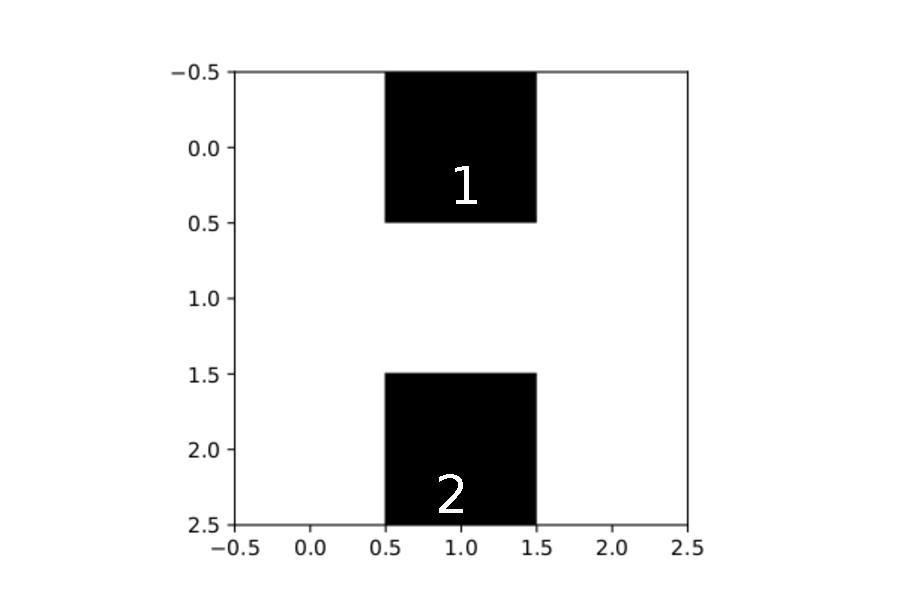
\includegraphics[scale=0.6]{noperc1.pdf}
	\caption{Es existiert offensichtlich kein perkolierender Cluster.}
\end{figure}

\vspace{0.5cm}
\noindent Würde man einfach das Labeln über periodische Randbedingung machen, würden beide Blöcke entsprechend Label 1 erhalten und nach dem Kriterium aus §1.2.2 hätte man einen perkolierenden Cluster gefunden. Dies ist ganz offensichtlich falsch, da es sich um einen Cluster endlicher Größe handelt.
\\
\noindent Der (scheinbar) korrekte Algorithmus den perkolierenden Cluster zu finden ist es, Cluster die sich über periodische Randbedinungen Berühren in einer Verlinkungsliste zu Speichern, zu den Labels muss die Richtung gespeichert werden. Man wählt die Konvention: links entspricht $(-1,0)$ rechts $(+1,0)$ unten $(0,-1)$ und oben entsprechend $(0,+1)$. Zu dem 'Weg' in der Verlinkungsliste muss die Summe der Richtungen gebildet werden, ist diese ungleich $(0,0)$ so perkolieren die Cluster die verlinkt sind. Man muss (rekursiv) eine Suchfunktion implementieren die alle zu einem gegebenen Label verlinkten Labels sucht. Auf alle Verlinkten Labels wird erneut die Suchfunktion angewendet, und so weiter, wird das Ausgangslabel gefunden so müssen die Richtungen addiert werden und mit $(0,0)$ verglichen werden.
\\
\noindent Am Beispiel der in Abbildung 4 gezeigten Matrix bedeuted die $1 \rightarrow 3$ hat Richtung $(+1,0)$, $3 \rightarrow 2$ bedeutet Richtung $(0,-1)$ und $2 \rightarrow 1$ wieder $(+1,0)$. Insgesamt hat dieser Weg also die Richtung $(+2,-1) \neq (0,0)$ und wird von dem Algorithmus gefunden.
\\
\noindent Im Gegensatz dazu zeigt die nächste Abbildung eine Matrix, mit einem $(0,0)$ Loop, man "läuft im Kreis", ohne das wirklich eine Box durchschritten wird. Diese Matrix wird auch nicht als perkolierend gefunden, eignet sich aber sehr gut zum debuggen.

\begin{figure}[h!]
	\centering
	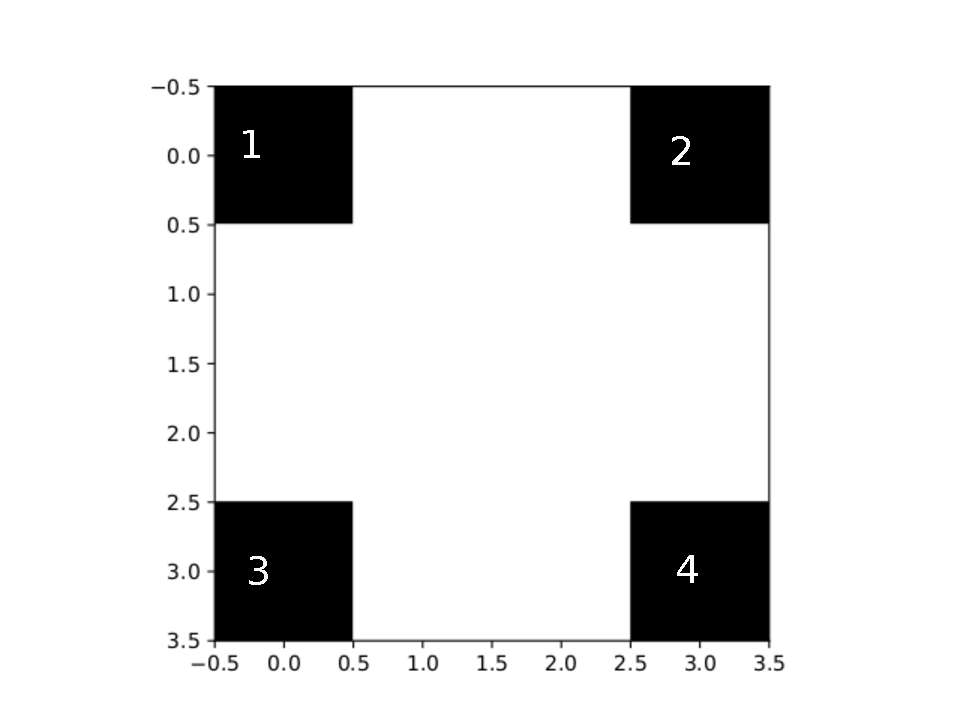
\includegraphics[scale=0.6]{noperc2.pdf}
	\caption{Es existiert offensichtlich kein perkolierender Cluster.}
\end{figure}

\noindent Das einzige Problem ist, dass dieser Algorithmus schlecht mit der Boxgröße skaliert, das die Anzahl der Labels quadratisch mit der Boxgröße skaliert und die Zahl der Knoten nochmals quadratisch mit der Boxgröße. Der Algorithmus skaliert also ungefähr mit $L^4$, wobei $L$ die Boxlänge bezeichnet. Unten sieht man den oben beschriebenen Teil zur Suche diagonal perkolierender Cluster als python Code, welcher auch in den nachfolgenden Simulationen genutzt worden ist.

\begin{figure}[h!]
	\centering
	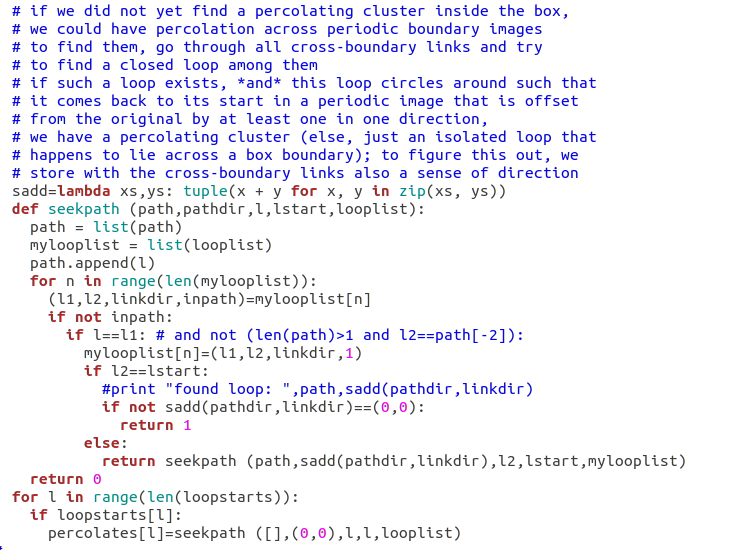
\includegraphics[scale=0.9]{diagcode.png}
	\caption{Python-Code zur Suche diagonal perkolierender Cluster.}
\end{figure}

\clearpage

\section{Random-Walk in ungeordneten Medien}

\subsection{"Normeler"\ Random-Walk}
Der (diskrete) Random-Walk auf dem freien Quadratgitter mit Hüpfwahrscheinlichkeit $\frac{1}{d}$ auf jeden der $d$ nächsten Nachbarn, wobei $d$ die Dimension des Gitter bezeichnet, unterliegt bekanntlich normaler Diffusion. Das heißt, dass das mittlere quadratische Verschiebung (engl. mean squared displacement), welches im weiteren mit $msd$ abgekürzt wird, linear mit der Anzahl an Schritten anwächst. Im kontinuierlichen Fall gilt die bekannte Formel:
\begin{align*}
msd(t)\equiv \langle \delta r^2 (t) \rangle =2dDt\ ,
\end{align*}
wobei (wie oben) $d$ die Dimension und $D$ der Diffusionskoeffizient sind, und hier gilt $D=1$.

\subsection{Random-Walk auf dem Perkolationsgitter}
Das Perkolationsgitter bei dem nur ein zufälliger Bruchteil der Gitterplätze begehbar sind und die anderen geblockt sind ist ein besonders einfaches Modell für ein ungeordnetes Medium. Eine spannende Frage - die in den 70er und 80er Jahren des vergangenen Jahrhunderts durch eine Vielzahl von Computersimulationen geklärt wurde - ist, wie sich ein Random-Walker auf so einem unregelmäßigen Perkolationgitter für verschiedene $p$ ($=$ Wahrscheinlichkeit das ein Gitterplatz begehbar ist) verhält. Speziell geht man, motiviert durch die fraktale Struktur der Cluster, von einem Potenzgesetz:
\begin{align*}
msd(t) \sim t^{2 \nu},\ \ \nu=1/d_w
\end{align*} 
aus, wobei $\nu$ als Diffusionsexponent bezeichnet wird und $d_w$ als 'walk dimension'. Der im Feld der weichen Materie bekannte französische Physiker Pierre-Gilles de Gennes nannte diese Fragestellung 1976 die 'Ameise im Labyrinth'.\footnote[2]{D. Stauffer, Perkolationstheorie, Kapitel 1.4} 
\\ 
\noindent Zuerst muss man die Hüpfwahrscheinlichkeiten festlegen, also ob $\frac{1}{f.n.N.}$ ($f.n.N.$ für freie nächste Nachbarn) oder wie bei dem freien Random-Walk $\frac{1}{d}$ und Züge auf ein geblocktes Feld werden zurückgesetzt. Für lange Zeiten sind beide Variaten äquivalent ('blind' vs 'myopic' ants)\footnote{S. Havlin and D. Ben-Avraham, Adv. Phys.36, 695 (1987), Appendix A.3}.\\
 Nun überlegt man sich leicht die beiden Extremfälle $p$ nahe $1$ und $p$ nahe $0$. Im ersten Fall ($p \approx 1$) erwartet man sofort, dass $\nu \rightarrow1/2$, da es kaum 'Hindernisse' gibt und der Random-Walk nahezu ungestört laufen kann. Anders herum, bei $p$ nahe $0$ erwartet man, dass es keine perkolierenden Cluster gibt, somit ist der Random-Walker 'eingesperrt' in sogenannte 'Taschen', damit das $msd$ beschränkt und somit $\nu \rightarrow 0$ für lange Zeiten. Besonders spannend ist dieses Problem also in der Nähe der Perkolationsschwelle $p=p_c$, hier findet sich ein Diffusionskoeffizient, der weder $1/2$ noch $0$ ist. Gefen, Aharony und Alexander nannten diesen Effekt, dass das $msd$ weder normal (linear, $\nu = 1/2$) mit $t$ anwächst noch beschränkt ist, sondern für lange Zeiten asymptotisch einem Potenzgesetz mit $\nu \neq 1/2$ folgt, 'anormale Diffusion'.\footnotemark[6] Diese anormale Diffusion wird, im Falle des unendlich großen Gitters, nur für $p=p_c$ gefunden, den für $p<p_c$ existiert kein perkolierender cluster, das $msd$ ist also beschränkt. Ist $p > p_c$ so gilt für $t \rightarrow \infty $ immer $msd \sim t$, aber es gibt ein 'Fenster' mit $msd \sim t^{2\nu}$, wobei $\nu < 1/2$ ist.

\newpage

\subsection{'all-cluster-' und 'percolating-cluster average'}

Es gibt im Allgemeinen zwei Varianten wie man $\nu_{pc}$ auffassen kann, man mittelt über zufällige Startpunkte auf dem zufällig geblockten Quadratgitter oder man mittelt über Startwerte die nur auf dem perkolierenden Cluster liegen ('all-cluster average' und \\ \noindent'percolating-cluster average'). Es ist zu erwarten, dass der Exponent bei dem 'all-cluster average' unter dem Exponenten des 'percolating-cluster average' liegt, da beim 'all-cluster average' auch in sogenannten Taschen gestartet wird in denen das $msd$ beschränkt ist. Die aktuell bekannten 'Literaturwerte' sind $d_w^{a.c.} \approx 3.036$ und $d_w^{p.c.} \approx 2.878$, woraus sich $\nu_{pc}^{a.c.} \approx 0.329$ und $\nu_{pc}^{p.c.} \approx 0.347$ ergeben.\footnote[4]{P. Grassberger, Phys. A 262, 251 (1999)} In dieser Spezialisierung wurde versucht diese Werte durch Monte-Carlo-Simulation (MC) zu reproduzieren. Es wurde eine Gitterlänge $L=1000$ verwendet und die Perkolationsschwelle als $p_c = 0.592\ 746$ angenommen. Es wurden zu beiden Mittelungsvarianten über $100$ Läufe auf je $100$ zufälligen Matrizen gemittelt, wobei nicht auf diagonale Perkolation getestet worden ist (aus Laufzeitgründen). Die Läufe waren je $10^6$ MC-Schritte lang und wurden auf einem ($10$er-) logarithmischen Grid gespeichert mit 48 Speicherstellen. 
\begin{figure}[h!]
\centering
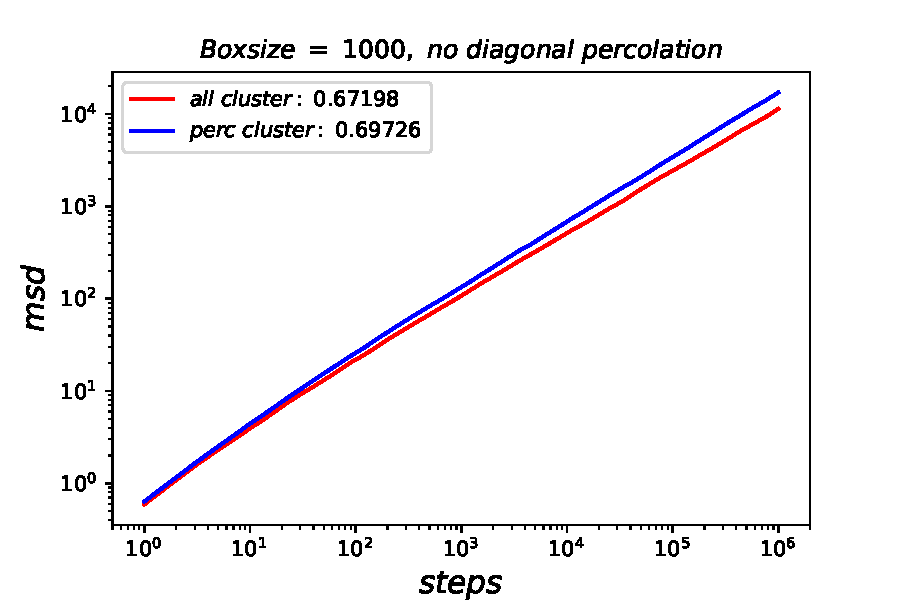
\includegraphics[scale=0.9]{acpcold1000.pdf}
\caption{Ergebnisse meiner python3 MC-Simulation, der 'all-cluster average' ist in rot, der 'percolating-cluster average' in blau, es wurden keine diagonal perkolierenden Cluster in die Statistik aufgenommen.}
\end{figure}
\vspace{0,5cm}
\newpage
\noindent Die Exponenten wurden über einen $scipy.optimize.curve\_fit$ als $2\nu_{pc}^{a.c.} \approx 0.6712$ und $2\nu_{pc}^{a.c.} \approx0.6973$ bestimmt. Die Methode den Exponenten durch einen fit zu bestimmen hat sich als deutlich stabiler herausgestellt als das bestimmen der Ableitung durch eine 'central-difference' oder 'forward-difference' Methode, welche unter sehr hohen numerischen Fehler leiden, da zwei sehr große Zahlen von einander abgezogen werden, deren Differenz klein ist. Dieses Problem ist bekannt als 'catastrophic cancellation'. Nimmt man Werte die weiter auseinander liegen (also ein größeres $h$), so wird die Ableitung ebenfalls sehr ungenau, da der Fehler quadratisch ('central-difference') beziehungsweise linear ('forward-difference') in Abstand $h$ wächst. Ein lokaler Mittelwert hilft etwas,
 die 'Zacken' in der numerischen Ableitung zu glätten, ist aber durch das logarithmische Grid mit Vorsicht zu genießen, da spätere Zeiten stärker gewichtet werden. Im nachfolgenden Plot ist die numerische Ableitung mit dem Fit-Parameter verglichen und ebenfalls die gefittete Kurve (in schwarz) an das 'all-cluster' mean-squared-displacement angelegt. Man erkennt, dass die numerische Ableitung, welche ähnlich zur 'central difference', aber auf einem logarithmischen Grid ist, und Fit übereinstimmen. Auf oben beschriebenes Glätten der Ableitung wurde verzichtet. 
\begin{figure}[h!]
	\centering
	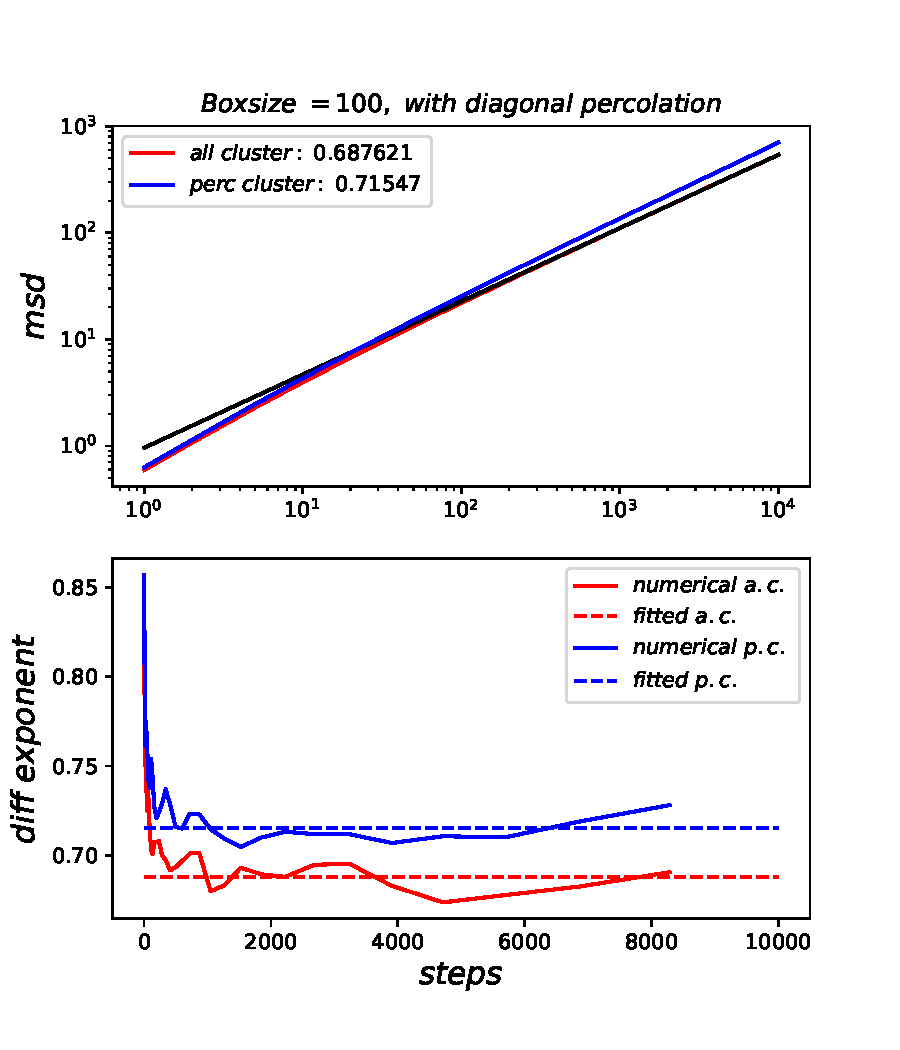
\includegraphics[scale=0.9]{newacpc100.pdf}
	\caption{Ergebnisse meiner python3 MC-Simulation, der 'all-cluster average' ist in rot, der 'percolating-cluster average' in blau, es wurden keine diagonal perkolierenden Cluster in die Statistik aufgenommen.}
\end{figure}
\newpage


\subsection{Vergleich der Statistik mit und ohne diagonale Perkolation}
\noindent In kleineren Simulationsboxen treten finite-size Effekte auf. Die Diffusionsexponenten sind weiter von den Literaturwerten für eine unendliche Box entfernt; dennoch sind (bei gleicher Boxgröße) wie nachfolgender Plot zeigt die Exponenten mit diagonal perkolierenden Clustern näher am Literaturwerten für eine unendliche Box. Es sind bei einer Boxgröße $L=100$ ca. $18,6\%$ der perkolierenden Cluster diagonal perkolierend. Größere Boxen sind aktuell durch zu hohe Laufzeit des Clustersuch-Algorithmus nicht (im Rahmen einer Spezialisierung) realisierbar.
\begin{figure}[h!]
	\centering
	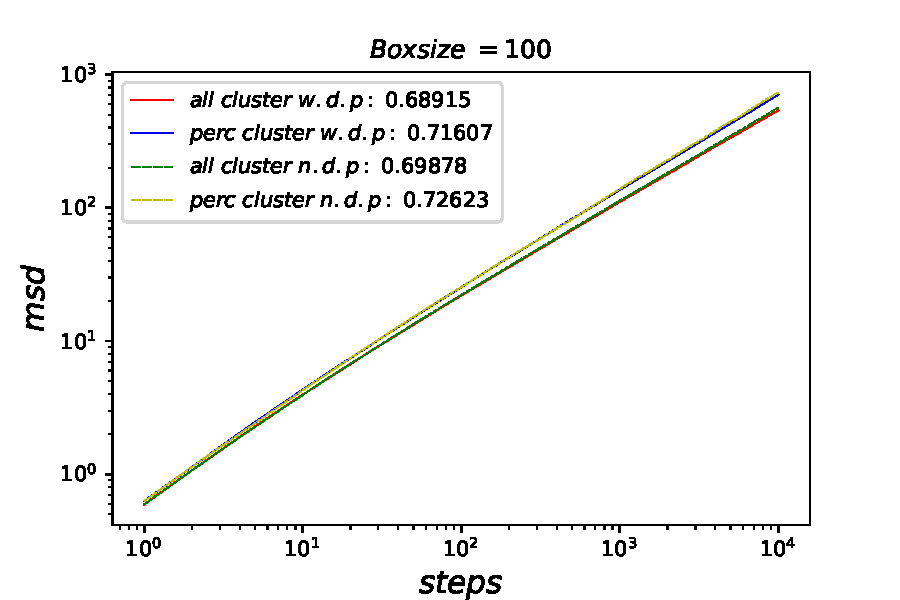
\includegraphics[scale=0.9]{both100.pdf}
	\caption{Vergleich von Statistik mit (w.d.p.) und ohne (n.d.p.) diagonal perkolierende Cluster. Gesamplet über 1000 Läufe auf je 500 Matrizen.}
\end{figure}

\noindent Man sieht vorallem an den Werten, das der Literaturwert von $2\nu_{pc}^{p.c.} \approx 0.694$ nun unterschätzt wird (bezogen auf den 'percolating-cluster average'). Zudem ist der Wert bei der Box mit Länge $L=1000$ ohne diagonal perkolierende Cluster näher am Literaturwert. Man sollte also lieber auf das finden der diagonal perkolierenden Cluster verzichten und größere Boxen wählen, denn der 'finite-size' Fehler scheint größer, als der Fehler, den das Auslassen der diagonal perkolierenden Cluster verursacht.
\subsection{Random-Walk auf diagonal perkolierenden Clustern}
Um den Einfluss der diagonal perkolierenden Cluster besser zu verstehen habe ich eine Simulation von 1000 Läufen auf je 500 diagonal perkolierenden Clustern angefertigt ('percolating-cluster average'). Die Boxgröße beträgt $L=100$. Es wurde $\nu_{pc}^{p.c.} \approx 0.681$ gefunden, dieser Wert unterschreitet den Literaturwert von $\nu_{pc}^{p.c.} \approx 0.694$. Dies ist leicht einzusehen, den diagonale Läufe haben ein geringeres $msd$, da ein Schritt nach (z.B.) rechts gefolgt von einem Schritt nach (z.B.) oben ein $msd$ von $2$ ergibt wohingegen zwei Schritte in eine Richtung ein $msd$ von $4$ ergeben. Die diagonal perkolierenden Cluster führen also auch dazu, dass das $msd$ geringer wird, so lässt sich erklären, das auch bei der Simulation der $L=1000$ Box in §2.3 beide Exponenten überschätzt werden.

\begin{figure}[h!]
	\centering
	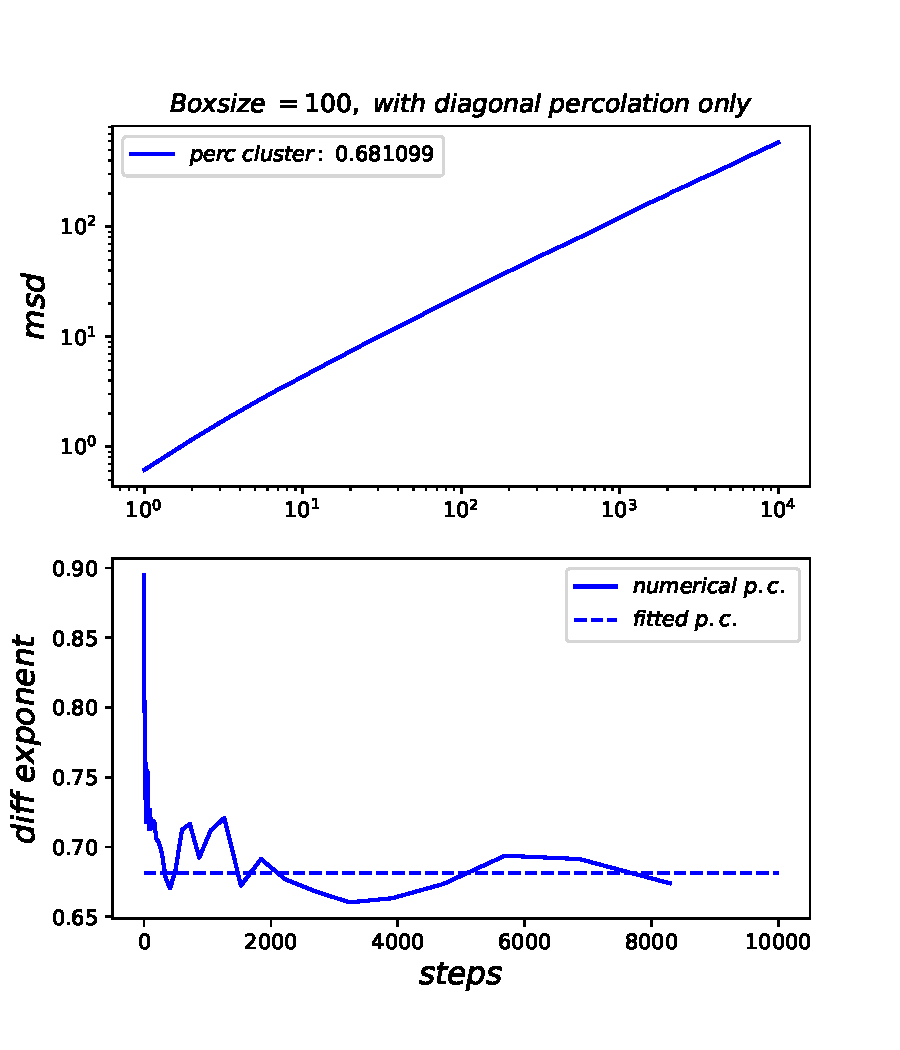
\includegraphics[scale=0.9]{diagpc100.pdf}
	\caption{Vergleich von Statistik mit und ohne diagonal perkolierende Cluster. Gesamplet über 1000 Läufe auf je 500 Matrizen.}
\end{figure}


\newpage


\subsection{Self-Avoiding Walk auf dem Perkolationsgitter}
Self-Avoiding Walks (kurz: SAW), also Random-Walks die niemals zu einem zuvor besuchten Gitterplatz zurückkehren sind ein Standardthema in der Physik der weichen Materie, da sie ein Modell für Polymerketten geben. Der Exponent $\nu^{SAW}$ des $msd$ beim SAW ist daher von besonderem Interesse, da er eine Verbingung zwischen mittlerer Größe eines Polymers und der Anzahl der Kettenglieder schafft:
\begin{align*}
\tilde R \equiv \sqrt{\langle R^2 \rangle} \sim N^{\nu^{SAW}},
\end{align*} 
wobei $\tilde R$ der Durchmesser des Polymers ist.
\\
Nun lässt sich auch leicht die Frage formulieren wie sich ein SAW auf dem Perkolationsgitter ausbreitet. Der normale Random-Walk ist langsamer geworden, genauer: $\nu_{pc} \equiv \nu_{pc}^{p.c.} < 1/2$, im Gegensatz dazu wird der SAW auf dem Perkolationsgitter schneller. In anderen Computersimulationen wurde $\nu^{pcSAW} \approx 0.78$ gefunden wohingegen $\nu^{SAW}=3/4=0.75$ ist\footnote[5]{V. Blavatska und W. Janke, Europhy. Lett. 82, 6606 (2008)}$^,$\footnote[6]{N. Fricke und W. Janke, Europhys. Lett. 99, 56005 (2012)}. Die Nachstehende Graphik zeigt, das auch endliche SAW sich auf dem p
Perkolationscluster schneller ausbreiten als auf dem freien Gitter\footnote[7]{Lee, Nakanishi und Kim, Phys. Rev. B 39, 13 (1989)} Der SAW ist ein wichtiger Vergleich zu dem 'aktiven' Random-Walk.
\begin{figure}[h!]
	\centering
	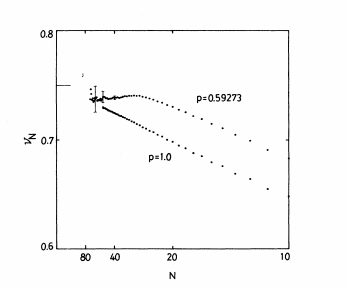
\includegraphics[scale=1.2]{saw.png}
	\caption{Ergebnisse einer MC-Simulation von Lee, Nakanishi und Kim. $N$ bezeichnet die Länge des SAW's.}
\end{figure}

\subsection{'Aktiver' Random-Walk auf dem Perkolationsgitter}
Es wird nun eine Variante des Random-Walk betrachtet, welche zuvor noch nicht besuchte Plätze bevorzugt. Diese Variante eines Random-Walks kann man zum Beispiel für die Modellierung von Chemotaxis von Bakterien verwenden. Das Modell sieht wie folgt aus: man generiert zuerst das Perkolationsgitter, danach werden begehbare Gitterplätze mit 'Nahrung' belegt, welche vom Random-Walker bei dem Besuch des jeweiligen Gitterplatzes vollständig 'gegessen' wird. Der Random-Walk erinnert also an 'Pacman' der durch ein Labyrinth (den perkolierenden Cluster) nach Nahrung absucht.
\begin{figure}[h!]
	\centering
	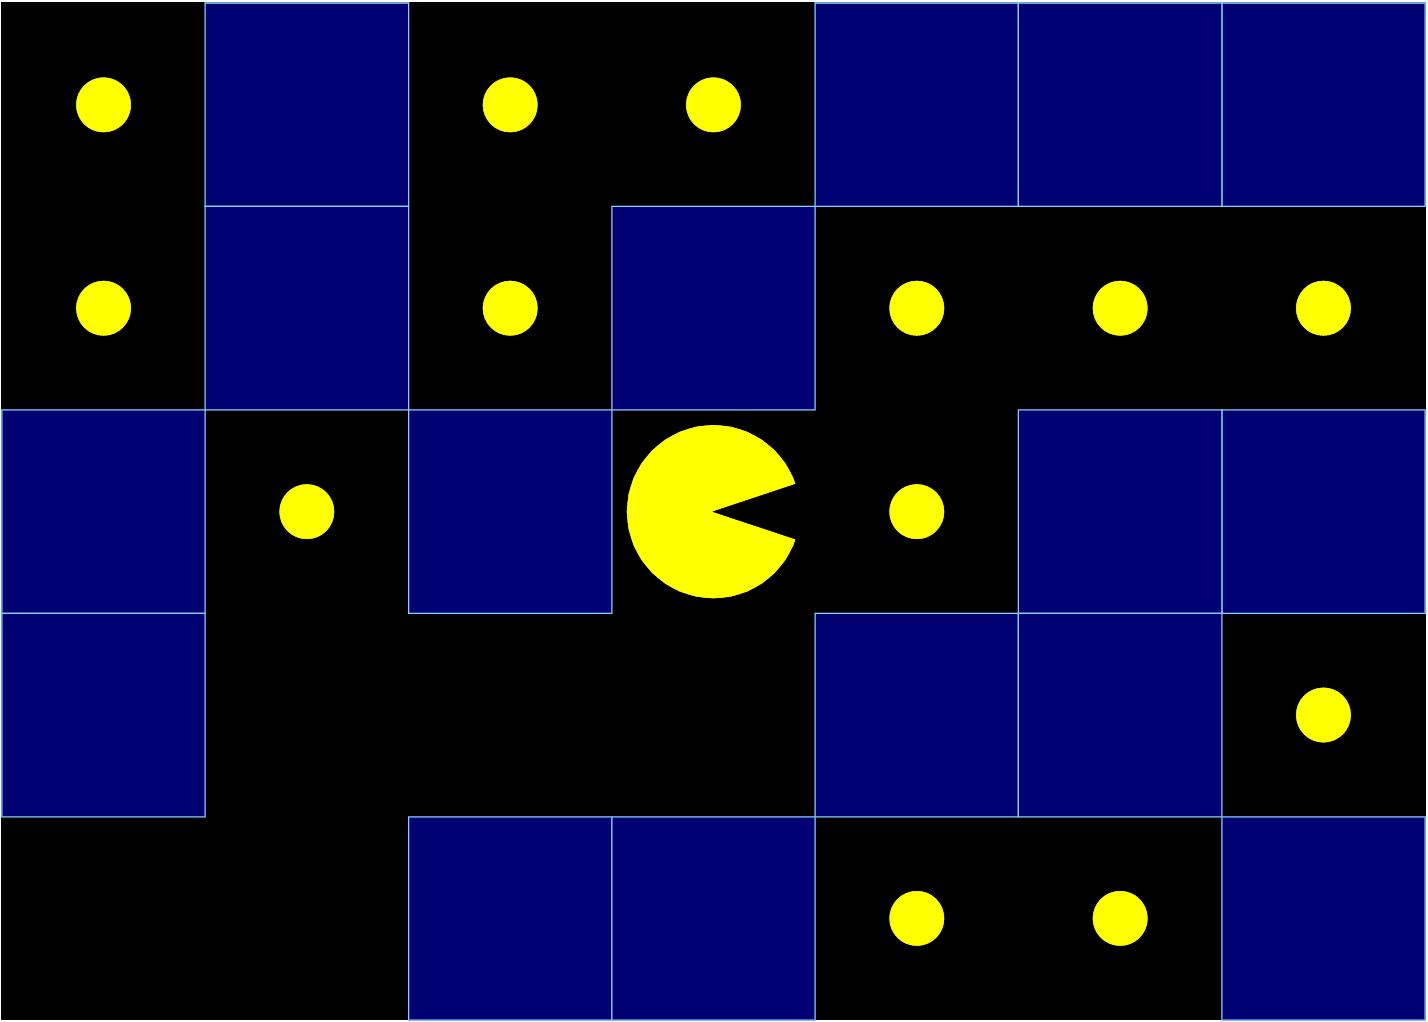
\includegraphics[scale=0.25]{pacman.png}
	\caption{Veranschaulichung des Modells, blaue Quadrate sind geblockte Gitterplätze, kleine gelbe Kreise sind Nahrung und 'Pacman' ist der Random-Walker.$^8$}
\end{figure}
\newpage


\noindent Die Wahrscheinlichkeiten für den nächsten Zug werden gemäß:
\begin{align}
	p_{j \leftarrow i} = \frac{exp({F_j})}{\sum_j exp({F_j})}
\end{align}
berechnet, wobei $F_j$ die Menge der Nahrung an Gitterplatz $j$ ist, also $F$ falls Gitterplatz $j$ noch nicht besucht worden ist und $0$ falls Gitterplatz $j$ zuvor bereits besucht wurde, $i$ ist dabei der Gitterplatz auf dem der Random-Walker aktuell ist. Dieses Modell scheint, insbesondere für $F \rightarrow \infty$, zuerst dem SAW sehr ähnlich zu sein, welcher auf dem Percolationsgitter schneller wird. Monte-Carlo-Simulation dieses 'aktiven' Random-Walkers auf dem Perkolationsgitter zeigt, das der Exponent kleiner ist, als der des normalen Random-Walkers auf dem Perkolationsgitter. Die Nachstehende Abbildung zeigt Ergebnisse einer Monte-Carlo-Simulation mit je $100$ Walks auf $100$ Perkolationsgittern (Matrizen), wobei nicht auf diagonale perkolation getestet worden ist, mit einer Größe von $1000 \times 1000$. Die Nahrung wird in meiner Simulation immer aus der Originalmatrix gelöscht und somit auch aus allen Kopien, welche durch die periodischen Randbedinungen entstehen, diese Methode ist zwar nicht ganz Korrekt (Quelle für finite-size-Effekte), führt aber zu keinem sichtbaren Fehler, solange die Wurzel aus dem $msd$ kleiner als die Boxgröße ist. Der Vorteil ist, dass diese Methode schneller ist und weniger Speicher benötigt. Die Perkolationsschwelle wurde wie zuvor als $p_c=0.592746$ angenommen.
\begin{figure}[h!]
	\centering
	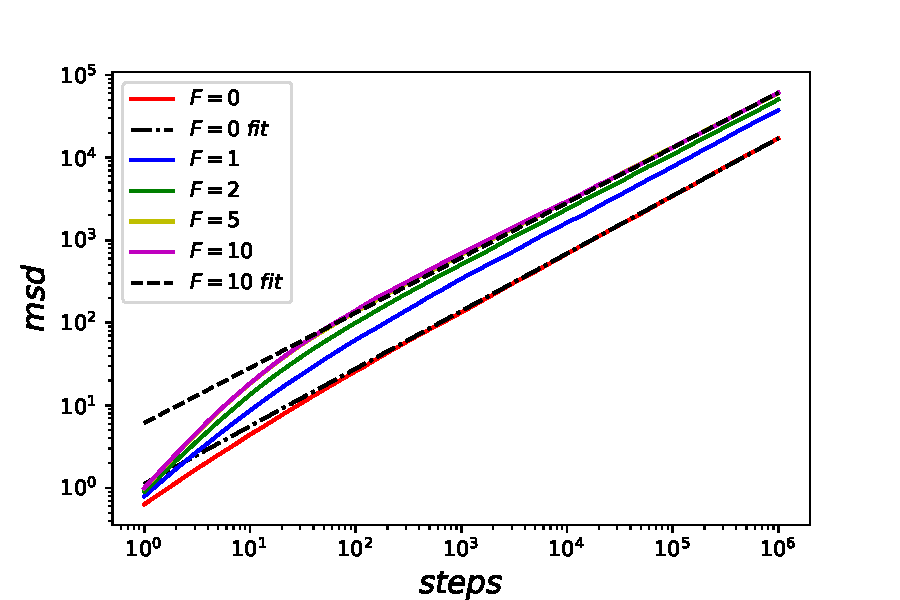
\includegraphics[scale=0.9]{food.pdf}
	\caption{Ergebnisse meiner python3 MC-Simulation des 'aktiven' Random-Walkers auf perkolierendem Cluster ohne diagonale Perkolation. Die gestrichelten Linien sind die mit scipy bestimmten langzeit power-laws.}
\end{figure}
\newpage

\noindent Es lässt sich erkennen, dass mit steigendem $F$ der Diffusionsexponent $\nu$, also die (halbe) Steigung der Kurve abnimmt, entgegen der naiven Annahme, das je größer $F$ ist, desto ähnlicher wird dieses Modell dem SAW.
Es wurden die folgenden Diffusionskoeffizienten gefunden:

\begin{tabular}[h]{l|c}
F & $2\nu(F)$\\
\hline
0 & 0.697\\
1 & 0.682\\
2 & 0.664\\
5 & 0.655\\
10 & 0.666\\
\end{tabular}

\noindent Das gleiche Verhalten wurde auch bei einer kleineren Box von $L=100$ gefunden. Es wurde über 1000 Läufe auf je 100 Perkolationsgittern (inklusive diagonaler Perkolation) gemittelt.
\begin{figure}[h!]
	\centering
	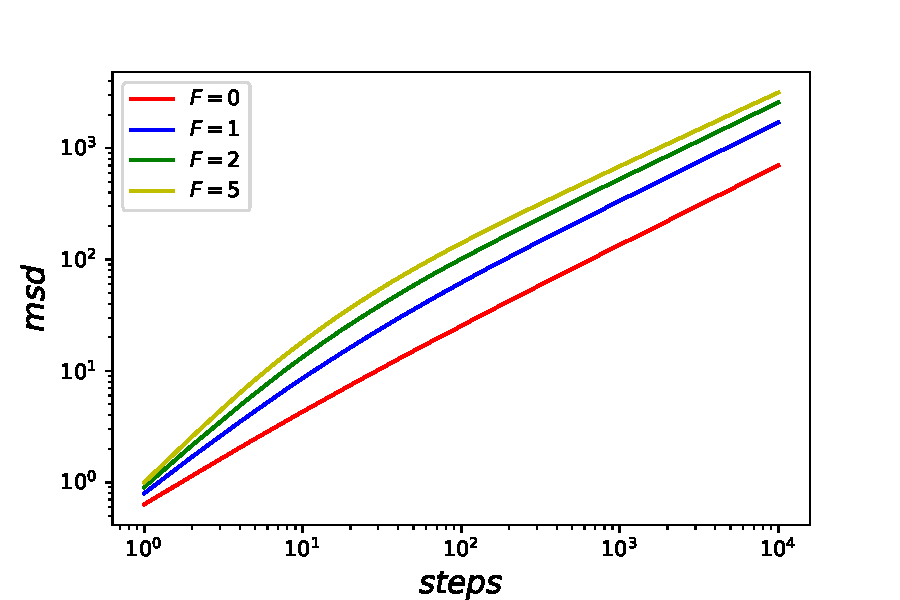
\includegraphics[scale=0.9]{newfood.pdf}
	\caption{Ergebnisse meiner python3 MC-Simulation des 'aktiven' Random-Walkers auf perkolierendem Cluster mit diagonaler Perkolation.}
\end{figure}
\newpage 
\noindent Erneut wurde die Nahrung die 'Pacman gegessen hat' aus der originalen Matrix und somit auch aus allen Kopien die durch die periodischen Randbedingungen entstehen gelöscht. Die Wurzel aus dem $msd$ ist erneut kleiner als die Boxlänge $L=100$.\\
\noindent Dieses Modell zeigt auch sehr schön den Unterschied zwischen fraktaler und Random-Walk Dimension, da das Perkolationsgitter (also die fraktale Dimension $\approx 1.7\ -\ 1.8$)\footnote[9]{R F Voss, J. Phys. A, 17, 7 (1984)} unabhängig von $F$ ist, die Random-Walk Dimension (also $1/\nu$) aber nicht.
\newpage
\noindent Monte-Carlo-Simulationen mit einer Boxgröße von $L=25000$ und bis zu $10^6$ Walks auf bis zu $100\ 000$ Matrizen zeigen das gleiche Verhalten. In diesen Simulationen\footnote[8]{T. Schilling und T. Voigtmann, J. Chem. Phys. 147, 214905 (2017)} wurden die bereits besuchten Gitterplätze korrekt mit einem 'hash-table' nachgehalten. Die Ergebnisse dieser MC-Simulationen befinden sich in der nachfolgenden Abbildung.

\begin{figure}[h!]
	\centering
	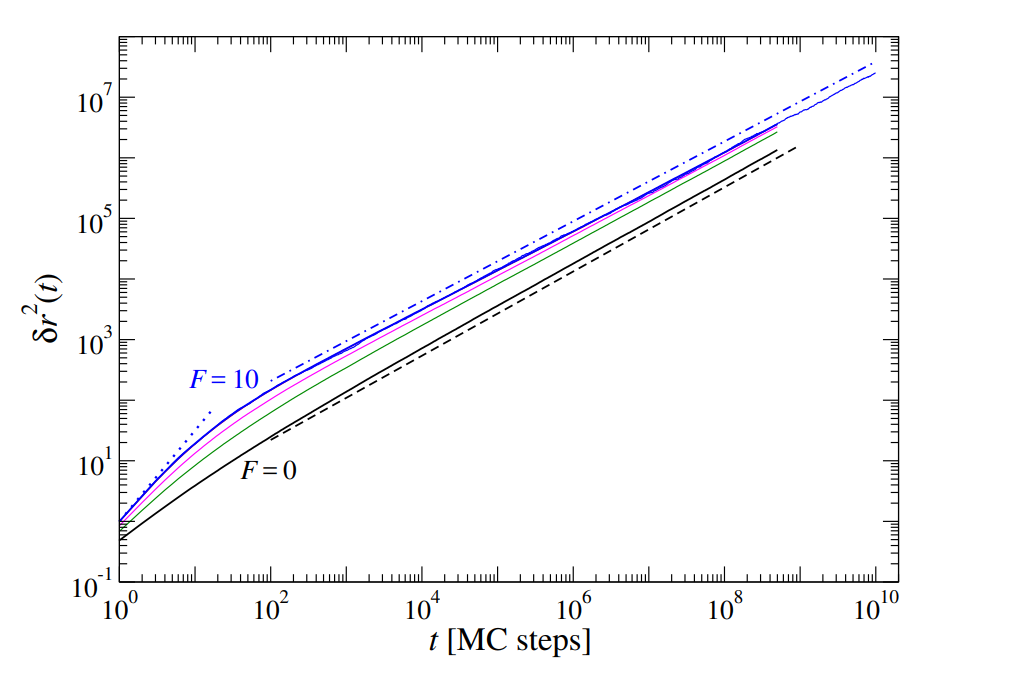
\includegraphics[scale=0.5]{food_thomas.png}
	\caption{Die blau gepunktete Linie zeigt die power-law des SAW ($\nu^{SAW}=3/4$), die blau gepunktet/gestrichelte Linie eine power-law zum Exponenten $\nu = 0.33$.}
\end{figure}

\end{document}